\documentclass[12pt,reqno]{amsart}
\usepackage[usenames, dvipsnames, svgnames]{xcolor}
\usepackage{amsmath, amssymb,graphicx,amsthm,latexsym, amsfonts, enumitem, mathtools, tensor, MnSymbol}
\usepackage[all, color]{xy}
\usepackage{color}
\usepackage{amssymb, wasysym}
\usepackage{tikz}
\usepackage{tikz-cd}
\usetikzlibrary{arrows,decorations.pathmorphing,decorations.pathreplacing,positioning,shapes.geometric,shapes.misc,decorations.markings,decorations.fractals,calc,patterns,}
\usepackage{circuitikz}
\usepackage{color}

\newcommand{\rectanglepath}{-- +(1cm,0cm)  -- +(1cm,1cm)  -- +(0cm,1cm) -- cycle}

\begin{document}

 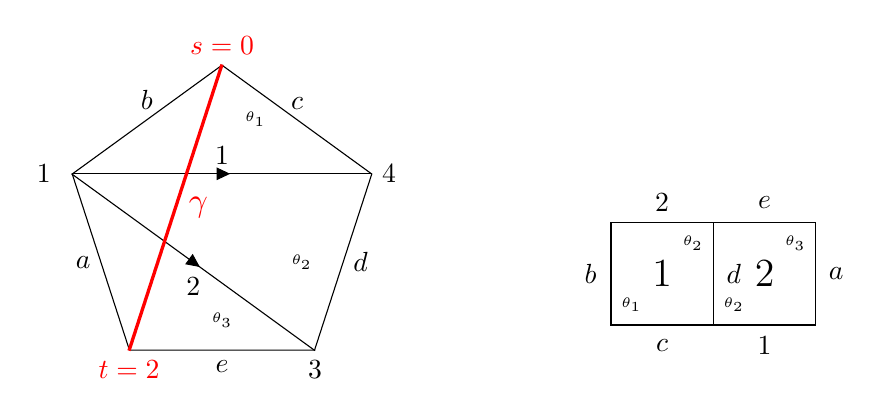
\begin{tikzpicture}
 \begin{scope}
   \node[draw,minimum size=4cm,regular polygon,regular polygon sides=5] (a) {};
  \draw  (a.corner 2)-- node[above] {$1$}  (a.corner 5)
  node[currarrow,pos=0.5, xscale=1, sloped]{};
  \draw  (a.corner 2)-- node[below=2pt] {$2$} (a.corner 4) node[currarrow,pos=0.5, xscale=1, sloped]{};
   \draw [color=red, very thick] (a.corner 1)-- node[right=.1pt,scale=1.2] {$\gamma$} (a.corner 3);
  \draw (a.corner 2) node[left=4pt]{$1$};
  \draw (a.corner 4) node[below]{$3$};
  \draw (a.corner 5) node[right]{$4$};
  \draw (a.corner 1) node[above,red]{$s=0$};
  \draw (a.corner 3) node[below,red]{$t=2$};
  \draw (a.side 3) node[below]{$e$};
  \draw (a.side 2) node[left]{$a$};
  \draw (a.side 1) node[above]{$b$};
  \draw (a.side 4) node[right]{$d$};
  \draw (a.side 5) node[above]{$c$};
  \draw (a.side 3) node[above=5pt]{\tiny $\theta_3$};
  \draw (a.side 5) node[left=8pt]{\tiny $\theta_1$};
  \draw (a.side 4) node[left=8pt]{\tiny $\theta_2$};
  \end{scope}
 \begin{scope}[scale=1.3, xshift=3.8cm, yshift=-1cm]
  \draw (0,0) \rectanglepath;
  \draw (1,0) \rectanglepath;
  \draw (-0.2,0.5) node{$b$};
  \draw (0.5,-0.2) node{$c$};
  \draw (1.5,-0.2) node{$1$};
  \draw (2.2,0.5) node{$a$};
  \draw (1.2,0.5) node{$d$};
  \draw (0.5,1.2) node{$2$};
  \draw (1.5,1.2) node{$e$};
  \draw (0.2,0.2) node{\tiny $\theta_1$};
  \draw (0.8,0.8) node{\tiny $\theta_2$};
  \draw (1.2,0.2) node{\tiny $\theta_2$};
  \draw (1.8,0.8) node{\tiny $\theta_3$};
   \draw (0.5,0.5) node{\Large $1$};
  \draw (1.5,0.5) node{\Large $2$};
 \end{scope}
 \end{tikzpicture}

\end{document}